% ============================================================
\chapter{NumPy I: vetores (\emph{arrays}) e cálculo numérico}
\label{cap:aula4}
% ============================================================

\begin{objetivos}
\begin{itemize}
  \item entender a diferença entre uma lista do Python e um \emph{array} do NumPy;
  \item criar \emph{arrays} com \py{np.array}, \py{np.zeros}, \py{np.ones}, \py{np.arange} e \py{np.linspace};
  \item fazer operações elemento a elemento e aplicar funções (\py{np.sin}, \py{np.exp}, ...) a vetores inteiros;
  \item selecionar elementos com índices, fatias e máscaras lógicas;
  \item usar somas, médias, máximos e somas acumuladas; aplicar a regra dos trapézios para integrais.
\end{itemize}
\end{objetivos}

\begin{roteiro}
0--10 min & Por que NumPy? Lista \emph{versus} \emph{array}.\\
10--25 min & Criando \emph{arrays}: \py{array}, \py{zeros}, \py{ones}, \py{arange}, \py{linspace}.\\
25--40 min & Operações elemento a elemento e funções universais; tabela de valores de uma função.\\
40--55 min & Índices, fatias e máscaras; \py{sum}, \py{mean}, \py{max}, \py{argmax}, \py{cumsum}.\\
55--75 min & Aplicações: séries, regra dos trapézios, Monte Carlo.\\
75--90 min & Exercícios.\\
\end{roteiro}

% ------------------------------------------------------------
\section{Por que NumPy?}
% ------------------------------------------------------------

O NumPy (\emph{Numerical Python}) é a biblioteca básica de computação científica em Python. Seu objeto principal é o
\textbf{\emph{array}} (vetor $n$-dimensional): uma sequência de números \emph{do mesmo tipo} com a qual se pode
fazer contas como se fosse um vetor da matemática. Por convenção, importa-se com o apelido \py{np}:

\begin{entrada}
import numpy as np

L = [1, 2, 3, 4]
v = np.array([1, 2, 3, 4])
print(L * 2)          # lista: repete
print(v * 2)          # array: multiplica cada elemento
print(L + [10])       # lista: concatena
print(v + 10)         # array: soma 10 a cada elemento
\end{entrada}
\begin{saida}
[1, 2, 3, 4, 1, 2, 3, 4]
[2 4 6 8]
[1, 2, 3, 4, 10]
[11 12 13 14]
\end{saida}

Repare que o \py{print} de um \emph{array} não tem vírgulas. Além de mais natural para a matemática, o NumPy é
muito mais rápido que as listas para grandes quantidades de números, pois as contas são feitas em código
compilado.

\begin{dica}
Se \py{import numpy} gerar \py{ModuleNotFoundError}, instale com \py{%pip install numpy} em uma célula do Jupyter
e reinicie o kernel.
\end{dica}

% ------------------------------------------------------------
\section{Criando \emph{arrays}}
% ------------------------------------------------------------

\begin{center}
\begin{tabular}{@{}ll@{}}
\toprule
\textbf{Comando} & \textbf{Resultado}\\
\midrule
\py{np.array([1, 2, 3])} & a partir de uma lista\\
\py{np.zeros(n)}, \py{np.ones(n)} & $n$ zeros / $n$ uns (\py{float})\\
\py{np.full(n, c)} & $n$ cópias do valor $c$\\
\py{np.arange(a, b, h)} & $a, a+h, a+2h, \dots$ (menores que $b$), como o \py{range}\\
\py{np.linspace(a, b, n)} & $n$ pontos igualmente espaçados de $a$ até $b$ (\textbf{inclui} $b$)\\
\bottomrule
\end{tabular}
\end{center}

\begin{entrada}
print(np.zeros(3), np.ones(4), np.full(3, 7))
print(np.arange(5))
print(np.arange(2, 9, 2))
print(np.arange(0, 1, 0.25))
print(np.linspace(0, 1, 5))
print(np.linspace(0, 10, num=5))
\end{entrada}
\begin{saida}
[0. 0. 0.] [1. 1. 1. 1.] [7 7 7]
[0 1 2 3 4]
[2 4 6 8]
[0.   0.25 0.5  0.75]
[0.   0.25 0.5  0.75 1.  ]
[ 0.   2.5  5.   7.5 10. ]
\end{saida}

\begin{figure}[ht]
\centering
\begin{tikzpicture}[x=11cm, font=\small]
  \draw[-{Stealth}] (-0.03,0) -- (1.06,0);
  \foreach \t in {0,0.25,0.5,0.75} { \fill[azul] (\t,0) circle (2.6pt); }
  \draw[vermelho, thick] (1,0) circle (3pt);
  \node[anchor=west, font=\ttfamily] at (1.07,0) {arange(0, 1, 0.25)};
  \node[below, font=\scriptsize] at (0,-0.1) {0};  \node[below, font=\scriptsize] at (1,-0.1) {1};
  \node[above, font=\scriptsize, text=azul] at (0.125,0.08) {passo $h=0{,}25$};
  \begin{scope}[yshift=-1.1cm]
  \draw[-{Stealth}] (-0.03,0) -- (1.06,0);
  \foreach \t in {0,0.25,0.5,0.75,1} { \fill[verde] (\t,0) circle (2.6pt); }
  \node[anchor=west, font=\ttfamily] at (1.07,0) {linspace(0, 1, 5)};
  \node[below, font=\scriptsize] at (0,-0.1) {0};  \node[below, font=\scriptsize] at (1,-0.1) {1};
  \node[above, font=\scriptsize, text=verde!70!black] at (0.5,0.08) {5 pontos, extremos incluídos};
  \end{scope}
\end{tikzpicture}
\caption{\texttt{arange} usa o \emph{passo} e exclui o fim; \texttt{linspace} usa a \emph{quantidade de pontos} e inclui o fim.}
\label{fig:arange-linspace}
\end{figure}

\begin{dica}
Para dividir um intervalo $[a,b]$ em pontos (para gráficos, tabelas e integrais), prefira \py{np.linspace}: com
passos decimais o \py{arange} pode incluir ou não o último ponto por causa de arredondamentos.
\end{dica}

Todo \emph{array} tem um tipo (\py{dtype}), uma forma (\py{shape}) e um tamanho (\py{size}):

\begin{entrada}
v = np.array([1, 2, 3])
w = np.array([1, 2.5, 3])
print(v.dtype, w.dtype, v.shape, v.size, v.ndim)
print(np.array([1, 2, 3], dtype=float))
\end{entrada}
\begin{saida}
int64 float64 (3,) 3 1
[1. 2. 3.]
\end{saida}

% ------------------------------------------------------------
\section{Operações elemento a elemento}
% ------------------------------------------------------------

As operações \py{+}, \py{-}, \py{*}, \py{/}, \py{**} entre \emph{arrays} do mesmo tamanho são feitas
\textbf{posição por posição}. Entre um \emph{array} e um número, o número é operado com cada elemento.

\begin{entrada}
u = np.array([1, 2, 3])
v = np.array([4, 5, 6])
print(u + v, u - v, u * v, v / u, u ** 2, 2 ** u)
print(np.dot(u, v), u @ v)       # produto escalar: 1*4 + 2*5 + 3*6
print(np.linalg.norm(u))         # norma: sqrt(1 + 4 + 9)
\end{entrada}
\begin{saida}
[5 7 9] [-3 -3 -3] [ 4 10 18] [4.  2.5 2. ] [1 4 9] [2 4 8]
32 32
3.7416573867739413
\end{saida}

\begin{atencao}
\py{u * v} \textbf{não} é o produto escalar: é o vetor dos produtos $(u_1v_1, u_2v_2, u_3v_3)$. O produto escalar
é \py{np.dot(u, v)} ou \py{u @ v}.
\end{atencao}

\subsection{Funções universais}

O NumPy tem suas próprias versões das funções matemáticas, que funcionam com \emph{arrays} inteiros:
\py{np.sqrt}, \py{np.exp}, \py{np.log}, \py{np.log10}, \py{np.sin}, \py{np.cos}, \py{np.tan},
\py{np.arcsin}, \py{np.arctan}, \py{np.abs}, \py{np.floor}, \py{np.ceil}, além das constantes \py{np.pi} e
\py{np.e}. Isso permite escrever uma função matemática e aplicá-la a muitos pontos de uma vez.

\begin{entrada}
x = np.linspace(0, np.pi, 5)
print(x)
print(np.sin(x))
print(np.round(np.sin(x), 4))
\end{entrada}
\begin{saida}
[0.         0.78539816 1.57079633 2.35619449 3.14159265]
[0.00000000e+00 7.07106781e-01 1.00000000e+00 7.07106781e-01
 1.22464680e-16]
[0.     0.7071 1.     0.7071 0.    ]
\end{saida}

% erro
\begin{entrada}
import math
math.sin(x)
\end{entrada}
\begin{saida}
TypeError: only 0-dimensional arrays can be converted to Python scalars
\end{saida}

As funções do \py{math} só aceitam \emph{um} número; para \emph{arrays}, use as do NumPy.

\paragraph{Tabela de valores.} Definindo uma função com operações do NumPy, ela pode receber um \emph{array}:

\begin{entrada}
def f(x):
    return x**2 * np.exp(-x)

x = np.linspace(0, 4, 9)
y = f(x)
for xi, yi in zip(x, y):
    print(f"{xi:5.2f}  {yi:8.5f}")
\end{entrada}
\begin{saida}
 0.00   0.00000
 0.50   0.15163
 1.00   0.36788
 1.50   0.50204
 2.00   0.54134
 2.50   0.51303
 3.00   0.44808
 3.50   0.36992
 4.00   0.29305
\end{saida}

Esse é exatamente o processo usado para fazer gráficos (Aula 6): calcula-se $f$ em muitos pontos e
ligam-se os pontos.

% ------------------------------------------------------------
\section{Índices, fatias e máscaras}
% ------------------------------------------------------------

Índices e fatias funcionam como nas listas (começando em 0). A novidade são as \textbf{máscaras}: uma condição
aplicada a um \emph{array} produz um \emph{array} de \py{True}/\py{False}, que pode ser usado para selecionar
elementos.

\begin{entrada}
v = np.array([3, -1, 4, -1, 5, -9, 2, 6])
print(v[0], v[-1], v[2:5], v[::2])
print(v > 0)
print(v[v > 0])                 # só os positivos
print(np.sum(v > 0))            # quantos são positivos (True conta 1)
v[v < 0] = 0                    # zera os negativos
print(v)
print(np.where(v > 3, 1, -1))   # 1 onde v > 3, -1 nos outros
\end{entrada}
\begin{saida}
3 6 [ 4 -1  5] [3 4 5 2]
[ True False  True False  True False  True  True]
[3 4 5 2 6]
5
[3 0 4 0 5 0 2 6]
[-1 -1  1 -1  1 -1 -1  1]
\end{saida}

Condições podem ser combinadas com \py{&} (``e'') e \py{|} (``ou''), \textbf{sempre entre parênteses}:

\begin{entrada}
n = np.arange(1, 31)
print(n[(n % 2 == 0) & (n % 3 == 0)])    # múltiplos de 2 e de 3
print(n[(n < 4) | (n > 27)])
\end{entrada}
\begin{saida}
[ 6 12 18 24 30]
[ 1  2  3 28 29 30]
\end{saida}

\begin{atencao}
Com \emph{arrays} não se usa \py{and}/\py{or}, e sim \py{&}/\py{|} com parênteses em cada condição.
\end{atencao}

% ------------------------------------------------------------
\section{Somas, médias e outras reduções}
% ------------------------------------------------------------

\begin{center}
\begin{tabular}{@{}ll@{}}
\toprule
\textbf{Comando} & \textbf{Resultado}\\
\midrule
\py{np.sum(v)}, \py{np.prod(v)} & soma e produto de todos os elementos\\
\py{np.mean(v)}, \py{np.std(v)}, \py{np.median(v)} & média, desvio padrão, mediana\\
\py{np.min(v)}, \py{np.max(v)} & menor e maior valor\\
\py{np.argmin(v)}, \py{np.argmax(v)} & \emph{índice} do menor e do maior valor\\
\py{np.cumsum(v)} & somas acumuladas $v_0,\ v_0+v_1,\ v_0+v_1+v_2, \dots$\\
\py{np.diff(v)} & diferenças $v_1-v_0,\ v_2-v_1,\dots$\\
\py{np.sort(v)} & cópia ordenada\\
\bottomrule
\end{tabular}
\end{center}

Também se pode escrever \py{v.sum()}, \py{v.mean()}, \py{v.max()} etc.

\begin{entrada}
notas = np.array([9.5, 7.5, 10, 8.0, 6.5])
print(notas.mean(), notas.std(), np.median(notas))
print(notas.max(), notas.argmax())
k = np.arange(1, 11)
print(np.cumsum(k))
print(np.diff(k**2))           # diferenças entre quadrados consecutivos
\end{entrada}
\begin{saida}
8.3 1.2884098726725126 8.0
10.0 2
[ 1  3  6 10 15 21 28 36 45 55]
[ 3  5  7  9 11 13 15 17 19]
\end{saida}

\paragraph{Máximo de uma função (aproximado).} Com um \emph{array} de muitos pontos, \py{argmax} dá o ponto onde
$f$ é maior. Para $f(x)=x^2e^{-x}$ em $[0,4]$, o máximo exato ocorre em $x=2$ (Aula 8):

\begin{entrada}
x = np.linspace(0, 4, 4001)
y = f(x)
i = np.argmax(y)
print(f"máximo aproximado em x = {x[i]:.4f}, f(x) = {y[i]:.6f}")
\end{entrada}
\begin{saida}
máximo aproximado em x = 2.0000, f(x) = 0.541341
\end{saida}

% ------------------------------------------------------------
\section{Aplicações}
% ------------------------------------------------------------

\subsection{Somas de séries sem laços}

Com \emph{arrays}, uma soma $\sum_{k=1}^{n} a_k$ se escreve em uma linha, sem \py{for}:

\begin{entrada}
k = np.arange(1, 100001)
print(np.sum(1 / k**2), np.pi**2 / 6)               # série de Basileia
j = np.arange(0, 100000)
print(4 * np.sum((-1)**j / (2*j + 1)), np.pi)        # série de Leibniz
\end{entrada}
\begin{saida}
1.6449240668982266 1.6449340668482264
3.1415826535897926 3.141592653589793
\end{saida}

As somas parciais (para ver a convergência) saem de \py{np.cumsum}:

\begin{entrada}
parciais = np.cumsum(1 / k**2)
for n in [10, 100, 1000, 10000, 100000]:
    print(n, parciais[n-1], np.pi**2/6 - parciais[n-1])
\end{entrada}
\begin{saida}
10 1.5497677311665408 0.09516633568168564
100 1.6349839001848923 0.009950166663334148
1000 1.6439345666815615 0.0009995001666649461
10000 1.6448340718480652 9.999500016122376e-05
100000 1.6449240668982423 9.999949984074163e-06
\end{saida}

O erro se comporta como $1/n$, o que se prova comparando a série com a integral $\int_n^\infty \frac{dx}{x^2}$.

\subsection{Integrais pela regra dos trapézios}

Para aproximar $\int_a^b f(x)\,dx$, dividimos $[a,b]$ em $n$ subintervalos de largura $h=\frac{b-a}{n}$, com pontos
$x_0=a, x_1,\dots,x_n=b$, e somamos as áreas dos trapézios:
\[
\int_a^b f(x)\,dx \approx h\left[\frac{f(x_0)}{2}+f(x_1)+\cdots+f(x_{n-1})+\frac{f(x_n)}{2}\right].
\]

\begin{figure}[ht]
\centering
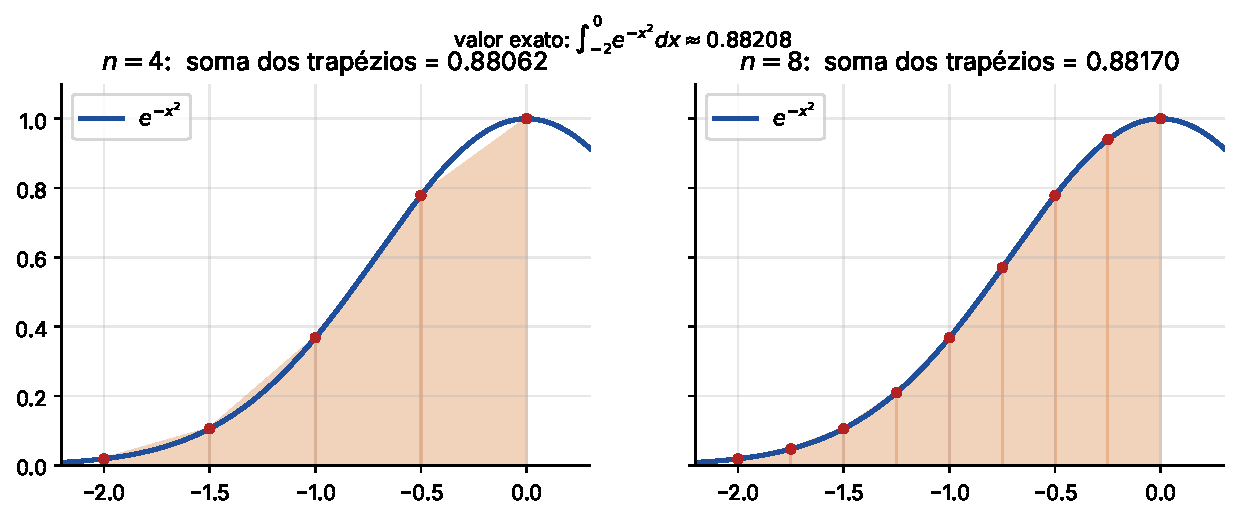
\includegraphics[width=0.95\linewidth]{aula04-trapezios}
\caption{Regra dos trapézios para $f(x)=e^{-x^2}$ em $[-2,0]$ com $n=4$ e $n=8$ subintervalos.}
\end{figure}

Seguindo o livro da SBM, calculamos $\int_{-\infty}^0 e^{-x^2}\,dx=\frac{\sqrt\pi}{2}$, aproximando $-\infty$ por
$-5$ (pois $e^{-25}\approx 10^{-11}$):

\begin{entrada}
def trapezios(f, a, b, n=100):
    x = np.linspace(a, b, n + 1)
    h = x[1] - x[0]
    y = f(x)
    return h * (np.sum(y) - (y[0] + y[-1]) / 2)

g = lambda x: np.exp(-x**2)
exato = np.sqrt(np.pi) / 2
for n in [10, 100, 1000]:
    I = trapezios(g, -5, 0, n)
    print(f"n = {n:5d}   I = {I:.12f}   erro = {abs(I - exato):.2e}")
\end{entrada}
\begin{saida}
n =    10   I = 0.886226925449   erro = 3.51e-12
n =   100   I = 0.886226925451   erro = 1.39e-12
n =  1000   I = 0.886226925451   erro = 1.38e-12
\end{saida}

Já com $n=10$ o resultado é excelente (isso acontece com funções muito ``suaves'' que se anulam nas pontas).
O erro que sobra, da ordem de $10^{-12}$, vem de termos trocado $-\infty$ por $-5$: a área desprezada é
$\int_{-\infty}^{-5}e^{-x^2}dx\approx 1{,}4\times10^{-12}$. Um exemplo mais típico é
$\int_0^1 \frac{4}{1+x^2}\,dx=\pi$:

\begin{entrada}
for n in [10, 20, 40, 80]:
    I = trapezios(lambda x: 4/(1 + x**2), 0, 1, n)
    print(f"n = {n:3d}   I = {I:.10f}   erro = {abs(I - np.pi):.2e}")
\end{entrada}
\begin{saida}
n =  10   I = 3.1399259889   erro = 1.67e-03
n =  20   I = 3.1411759870   erro = 4.17e-04
n =  40   I = 3.1414884869   erro = 1.04e-04
n =  80   I = 3.1415666119   erro = 2.60e-05
\end{saida}

Cada vez que $n$ dobra, o erro cai para $\frac14$: o erro da regra dos trapézios é proporcional a $h^2$.

\begin{observacao}
O NumPy já tem a regra dos trapézios pronta: \py{np.trapezoid(y, x)} (em versões antigas, \py{np.trapz}).
\end{observacao}

\subsection{Números aleatórios: estimando $\pi$ por Monte Carlo}

Sorteando pontos $(x,y)$ uniformemente no quadrado $[0,1]\times[0,1]$, a proporção dos que caem dentro do quarto
de círculo $x^2+y^2\le 1$ se aproxima da razão entre as áreas, $\frac{\pi/4}{1}$.

\begin{figure}[ht]
\centering
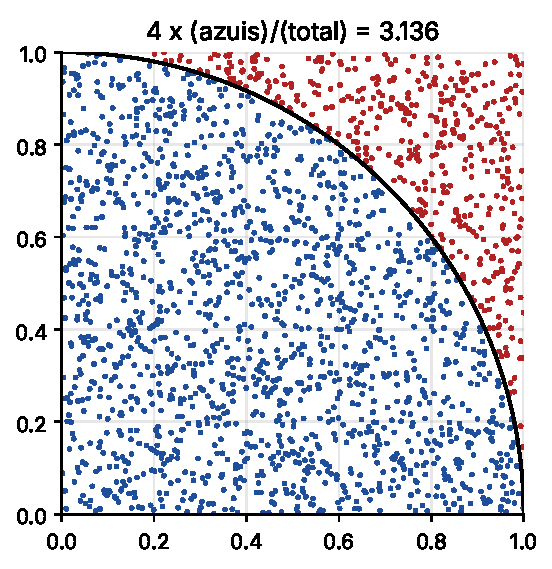
\includegraphics[width=0.42\linewidth]{aula04-montecarlo}
\caption{2000 pontos sorteados: em azul, os que caem dentro do quarto de círculo.}
\end{figure}

\begin{entrada}
rng = np.random.default_rng(2024)      # gerador com "semente" fixa
for n in [100, 10_000, 1_000_000]:
    x = rng.random(n)
    y = rng.random(n)
    dentro = np.sum(x**2 + y**2 <= 1)
    print(f"n = {n:8d}   pi ~ {4 * dentro / n:.5f}")
\end{entrada}
\begin{saida}
n =      100   pi ~ 3.36000
n =    10000   pi ~ 3.13760
n =  1000000   pi ~ 3.14259
\end{saida}

(Com outra semente os valores mudam; o erro típico é da ordem de $1/\sqrt{n}$.)

\subsection{Notação científica}

\begin{entrada}
c = (12 - 3)**100 * 100**100
print(np.format_float_scientific(c, precision=4))
print(f"{float(c):.4e}")
\end{entrada}
\begin{saida}
2.6561e+295
2.6561e+295
\end{saida}

\begin{professor}
O exemplo de Monte Carlo é uma boa oportunidade para discutir o que é uma ``semente'' e por que resultados
aleatórios variam. Se o tempo permitir, peça aos alunos que troquem a semente e comparem os resultados entre si.
\end{professor}

% ------------------------------------------------------------
\section{Exercícios}
% ------------------------------------------------------------

\begin{exercicio}[criando arrays]{ex:4-criar}
Crie, sem usar \py{for}: (a) os 20 primeiros ímpares; (b) 11 pontos igualmente espaçados em $[-1,1]$;
(c) as potências $2^0, 2^1,\dots,2^{10}$; (d) o vetor $\left(1,\frac12,\frac13,\dots,\frac1{10}\right)$.
\end{exercicio}

\begin{exercicio}[tabela]{ex:4-tabela}
Faça uma tabela de $\sin x$, $\cos x$ e $\sin^2x+\cos^2x$ para 7 pontos igualmente espaçados em $[0, \pi]$.
\end{exercicio}

\begin{exercicio}[estatística]{ex:4-estat}
Dadas as alturas (em m) \py{h = np.array([1.72, 1.65, 1.80, 1.58, 1.75, 1.69, 1.83, 1.61])}: calcule a média, o
desvio padrão, quantas pessoas têm mais de 1{,}70\,m e a média apenas dessas pessoas.
\end{exercicio}

\begin{exercicio}[série harmônica]{ex:4-harmonica}
Usando \py{np.cumsum}, encontre o menor $n$ tal que $1+\frac12+\cdots+\frac1n>10$. Compare
$\sum_{k=1}^n\frac1k - \ln n$ para $n=10^6$ com a constante de Euler--Mascheroni $\gamma\approx0{,}5772$.
\end{exercicio}

\begin{exercicio}[regra de Simpson]{ex:4-simpson}
A regra de Simpson (com $n$ par) é
\[\int_a^b f\approx \frac h3\left[f(x_0)+4f(x_1)+2f(x_2)+4f(x_3)+\cdots+4f(x_{n-1})+f(x_n)\right].\]
Implemente-a usando fatias (\py{y[1:-1:2]} e \py{y[2:-1:2]}) e compare com os trapézios em
$\int_0^1\frac{4}{1+x^2}dx$ para $n=10, 20, 40$.
\end{exercicio}

\begin{exercicio}[extra: Monte Carlo para integrais]{ex:4-mc}
Se $x_1,\dots,x_n$ são sorteados uniformemente em $[0,1]$, então $\frac1n\sum f(x_i)\approx\int_0^1 f$. Use isso
para estimar $\int_0^1 e^{-x^2}dx$ e compare com a regra dos trapézios.
\end{exercicio}
